\documentclass{anstrans}
%%%%%%%%%%%%%%%%%%%%%%%%%%%%%%%%%%%
\title{Full-core analysis of thorium-fueled molten salt breeder reactor using the SERPENT-2 Monte Carlo code}

\author{Andrei Rykhlevskii, Kathryn Huff, Alexander Lindsay}

\institute{
Department of Nuclear, Plasma, and Radiological Engineering, University of Illinois at Urbana-Champaign \break
Urbana, IL
}

\email{andreir2@illinois.edu}

%%%% packages and definitions (optional)
\usepackage{graphicx} % allows inclusion of graphics
\usepackage{caption}  % allows center figures caption
\usepackage{booktabs} % nice rules (thick lines) for tables
\usepackage{microtype} % improves typography for PDF
\graphicspath{{figures/}}

\newcommand{\SN}{S$_N$}
\renewcommand{\vec}[1]{\bm{#1}} %vector is bold italic
\newcommand{\vd}{\bm{\cdot}} % slightly bold vector dot
\newcommand{\grad}{\vec{\nabla}} % gradient
\newcommand{\ud}{\mathop{}\!\mathrm{d}} % upright derivative symbol

\begin{document}
%%%%%%%%%%%%%%%%%%%%%%%%%%%%%%%%%%%%%%%%%%%%%%%%%%%%%%%%%%%%%%%%%%%%%%%%%%%%%%%%
\section{1. Introduction}
The molten salt reactor (MSR) is advanced type of reactor which was  developed at Oak Ridge National Laboratory for a military aircraft nuclear propulsion project. In the MSR fluorides of fissile and/or fertile materials (i.e. $UF_4$, $PuF_3$ and/or $ThF_4$) are mixed with carrier salts to form a liquid fuel which circulated in a loop-type primary circuit \cite{haubenreich_experience_1970}. This conception leads to immediate advantages over traditional reactors with a solid fuel, such as near-atmospheric pressure in the primary loop, relatively high coolant temperature, outstanding neutron economy, a high level of inherent safety, reduced fuel preprocessing, and the ability to continuously remove fission products and add fissile and/or fertile elements \cite{leblanc_molten_2010}. 

Thermal spectrum Molten Salt Breeder Reactor (MSBR) designed specifically to realize promising thorium fuel cycle which allows use natural thorium instead of enriched uranium as the fertile element to breed the fissile $^{233}U$ and avoid uranium enrichment. The mixtures of $LiF-BeF_2-ThF_4-UF_4-PuF_3$ (72-16-12-0.232-0.0006 mole \%) has a melting point $499^\circ$C, good flow and heat transfer properties \cite{robertson_conceptual_1971}.

For the development of MSBR research, this paper demonstrates advanced whole-core three-dimensional model developed using a continuous-energy Monte Carlo reactor physics calculation code Serpent 2 and cross-verification with existing MCNP6 results \cite{park_whole_2015,leppanen_serpent_2012}. The neutronics model could be useful for optimization fuel salt composition and fuel utilization, neutron fluxes and spectrum evaluation, and for depletion calculations using built-in Serpent burnup module. Moreover, this model in the future will be employed to generate problem-oriented homogenized nuclear data (multi-group cross sections and diffusion constants) for deterministic reactor codes, multi-physics simulations \cite{fridman_use_2011,valtavirta_coupled_2017} as well as for routine applications.

All the calculations presented in this paper were performed using the Serpent 2 code version 2.1.28. Comparing with Serpent 1, Serpent 2 has many more useful features and contains a complete redesign of memory management using hybrid OpenMP + MPI parallelization, which is important in depletion calculations using computer clusters with multiple cores \cite{leppanen_serpent_2015}. Before burnup calculations can be undertaken MSBR model should be validated. In Section 2 a brief description of the MSBR geometry model is given. In Section 3 the results are presented and discussed. Section 4 reflected conclusions and plans for the future research.

%%%%%%%%%%%%%%%%%%%%%%%%%%%%%%%%%%%%%%%%%%%%%%%%%%%%%%%%%%%%%%%%%%%%%%%%%%%%%%%%
\section{2. MSBR design description}
MSBR vessel has diameter 680 cm and high 610 cm and contains molten fluoride fuel-salt mixture which performs to functions: generate heat in the moderated region and transport heat energy from the core to primary heat exchanger using primary salt pump. The vessel also contains graphite blocks for neutron moderation and reflection. The reactor core has a central zone, Zone I, in which 13\% of the volume is fuel salt and 87\% - graphite. The first zone is composed of 1320 graphite cells, 2 graphite control rods and 2 safety rods consisting of boron carbide clad. 

The undermoderated zone, Zone II, with 37\% fuel salt, or radial reflector, surrounding the more active portion serves to diminish neutron leakage from the reactor core. This zone is formed of two kinds of elements: elements like those for Zone I except for a larger hole size (Zone II-A), and radially spread graphite slats (Zone II-B). At the outer of the core there are 70cm-thick graphite reflector and 5cm-thick vessel wall. Betweeen the core and the reflector blocks located 5.08cm-wide annulus which is 100\% salt needed to provide possibility removing and inserting a core graphite assembly. 

Figure~\ref{fig:plan} shows plan view of the whole core configuration at the expected reactor operational level when all control rods are fully withdrawn from the core.  Figure~\ref{fig:elevation} shows longitudinal section of the reactor. The violet color represents bare graphite, and the yellow represents fuel salt. The blue color shows Hastelloy-N, material used for the plenum and vessel wall, and the black color is a void space. All figures of the core in this work generated using built-in Serpent plotter.
\begin{figure}[ht] % replace 't' with 'b' to force it to be on the bottom
  \centering
  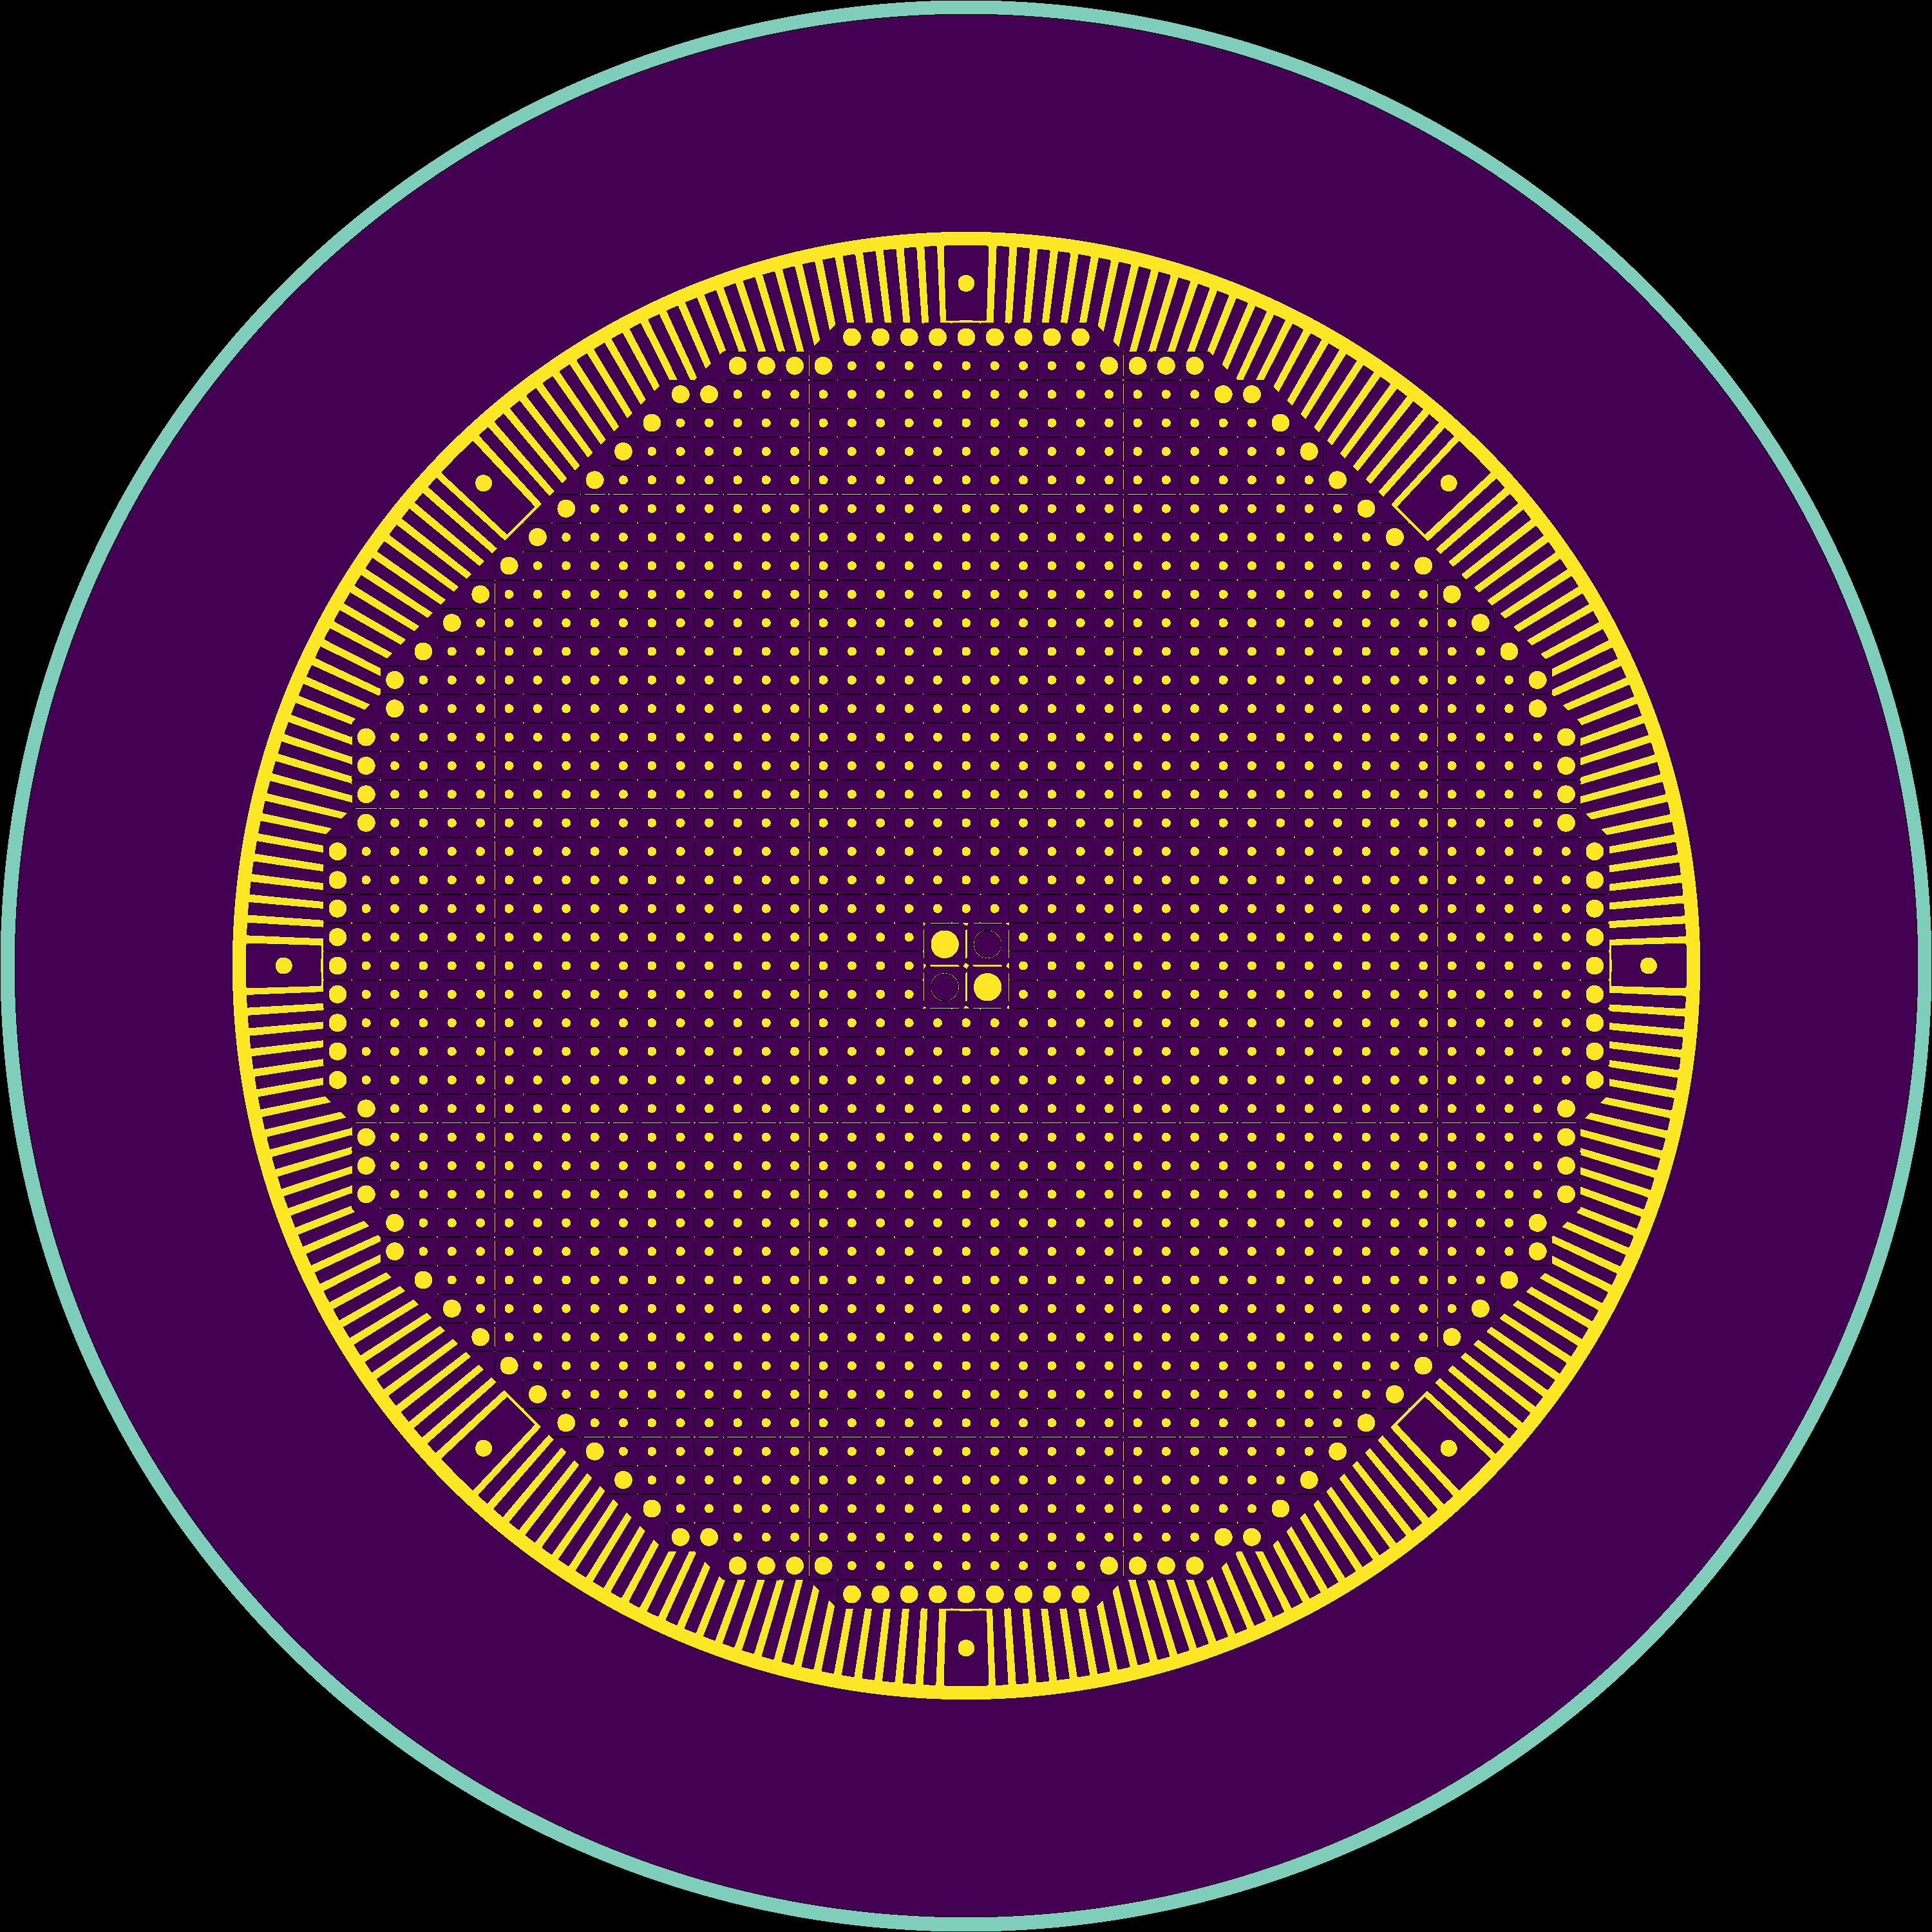
\includegraphics[width=\linewidth]{figure_2_1.png}
  \caption{Plan view of molten salt breeder reactor (MSBR) core.}
  \label{fig:plan}
\end{figure}

\begin{figure}[ht] % replace 't' with 'b' to force it to be on the bottom
  \centering
  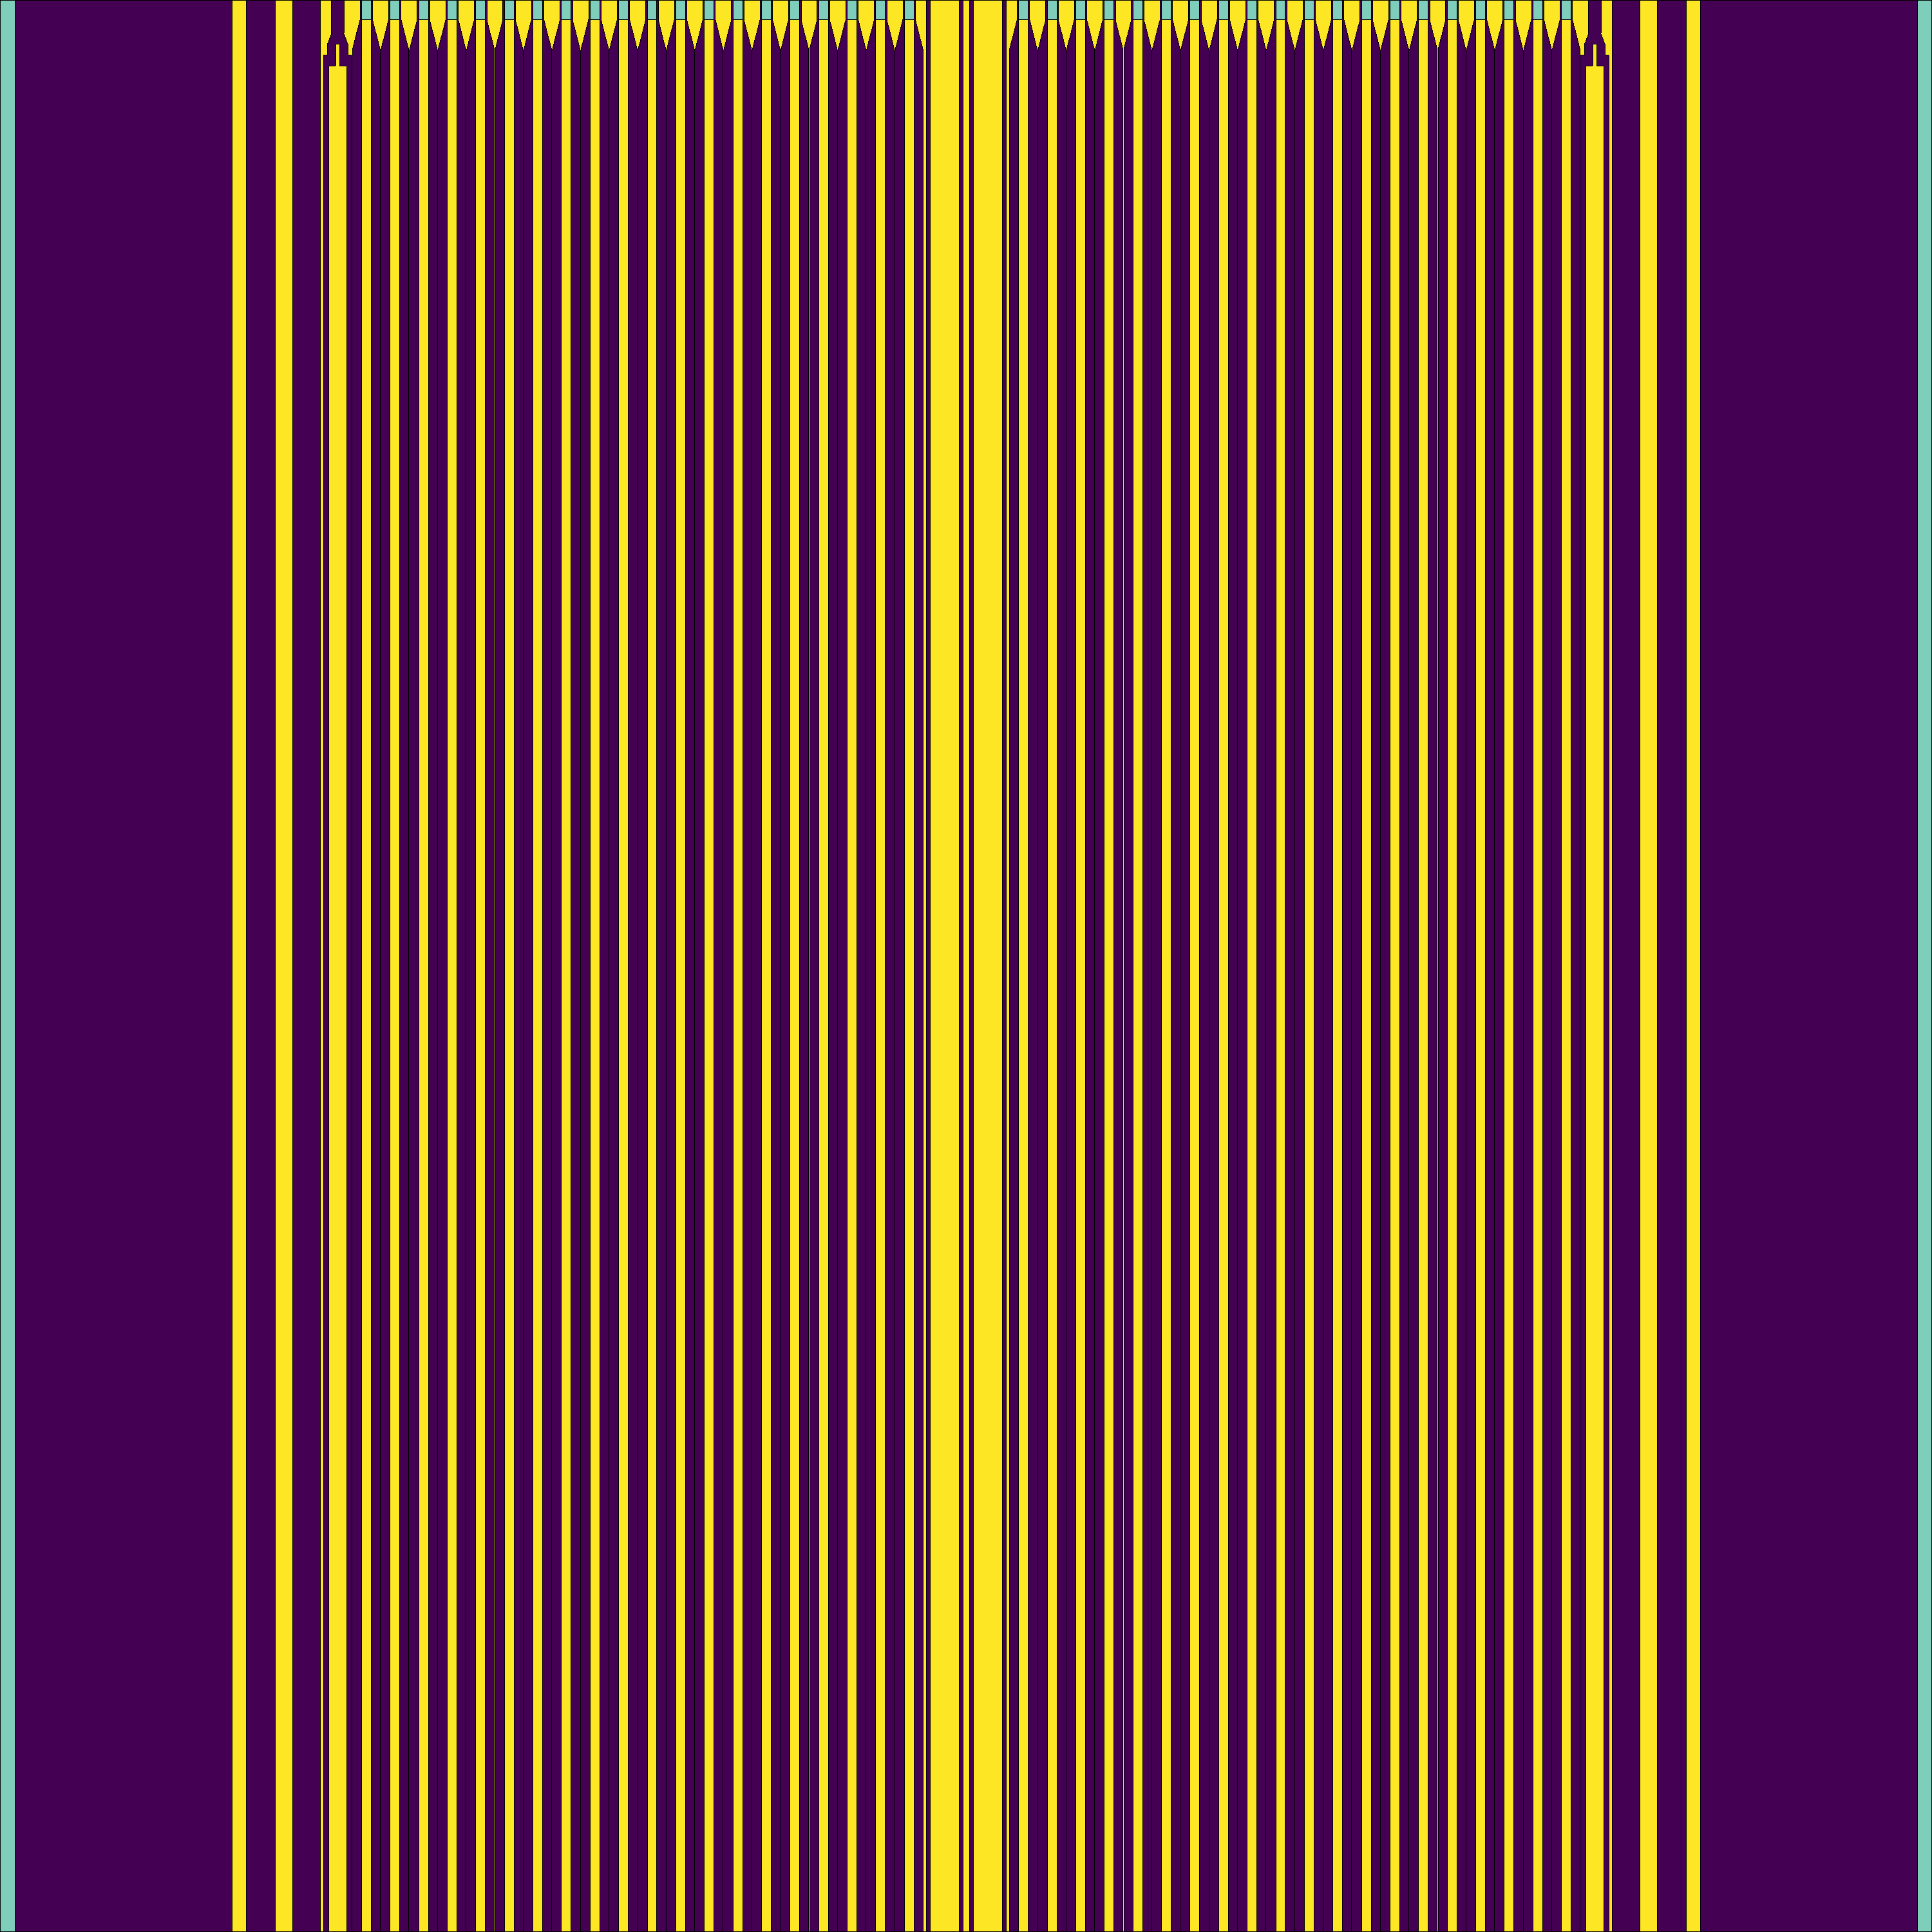
\includegraphics[width=\linewidth]{figure_2_2.png}
  \caption{Elevation view of molten salt breeder reactor (MSBR).}
  \label{fig:elevation}
\end{figure}

\subsection{2.1. Zone I and II-A}
The central portion, called Zone I, is made up of $10.16cm\times10.16cm\times396.24cm$-long graphite elements. The fuel salt to graphite volume ratio of Zone 1 is 13.2\% which possible with a central hole diameter about $3.42cm$. Zone II having 37\% salt and central hole diameter about $6.604cm$. Both types of elements mostly have rectangular shape with a part of cylinder sticking out at each corner to form salt flow between tje griphite channels. Different sizes of elements neccesarily to reduce the peak damage flux and power density in the center of the core to prevent local graphite damage. Figure~\ref{fig:zone12A} demonstrates the reconstructed graphite element utilized for Serpent model.

\begin{figure}[h] % replace 't' with 'b' to force it to be on the bottom
  \centering
  
\includegraphics[width=0.95\linewidth]{figure_2_4.png}
  \caption{Zone I (left) and Zone II-A (right) elements.}
  \label{fig:zone12A}
\end{figure}

\subsection{2.2. Zone II-B}
Second core zone is divided into two different zones: Zone II-A and Zone II-B. The graphite elements for zone II-A are prismatic and form first reflecting layer surrounding the core zone I. The elements for zone II-B made ip in the foru of rectangular slats spaced far enough apart to achieve 0.37 fuel salt volume fraction. Figure~\ref{fig:zone2B} shows Zone II, 5.08cm-wide annular space between the core graphite and the radial reflector graphite. The annulus contains 100\% fuel salt and serves to reduce the damage flux for internal surface of the graphite reflector blocks. From the ORNL report suggested model for Zone II-B has 8 graphite elements every $45^\circ$ with special shape and have holes for the flow of salt and were simplified into a uniformly sized chopped fan shape with the central hole. All other graphite $5.08cm$-thick slats and various length in width (average width is about $26.67cm$ are reconstructed as is in the model without any approximation.


%%%%%%%%%%%%%%%%%%%%%%%%%%%%%%%%%%%%%%%%%%%%%%%%%%%%%%%%%%%%%%%%%%%%%%%%%%%%%%%%
\section{3. Results and Analysis}
The results were interesting, so interesting in fact that we have decided to
present them here.

\begin{figure}[ht] % replace 't' with 'b' to force it to be on the bottom
  \centering
  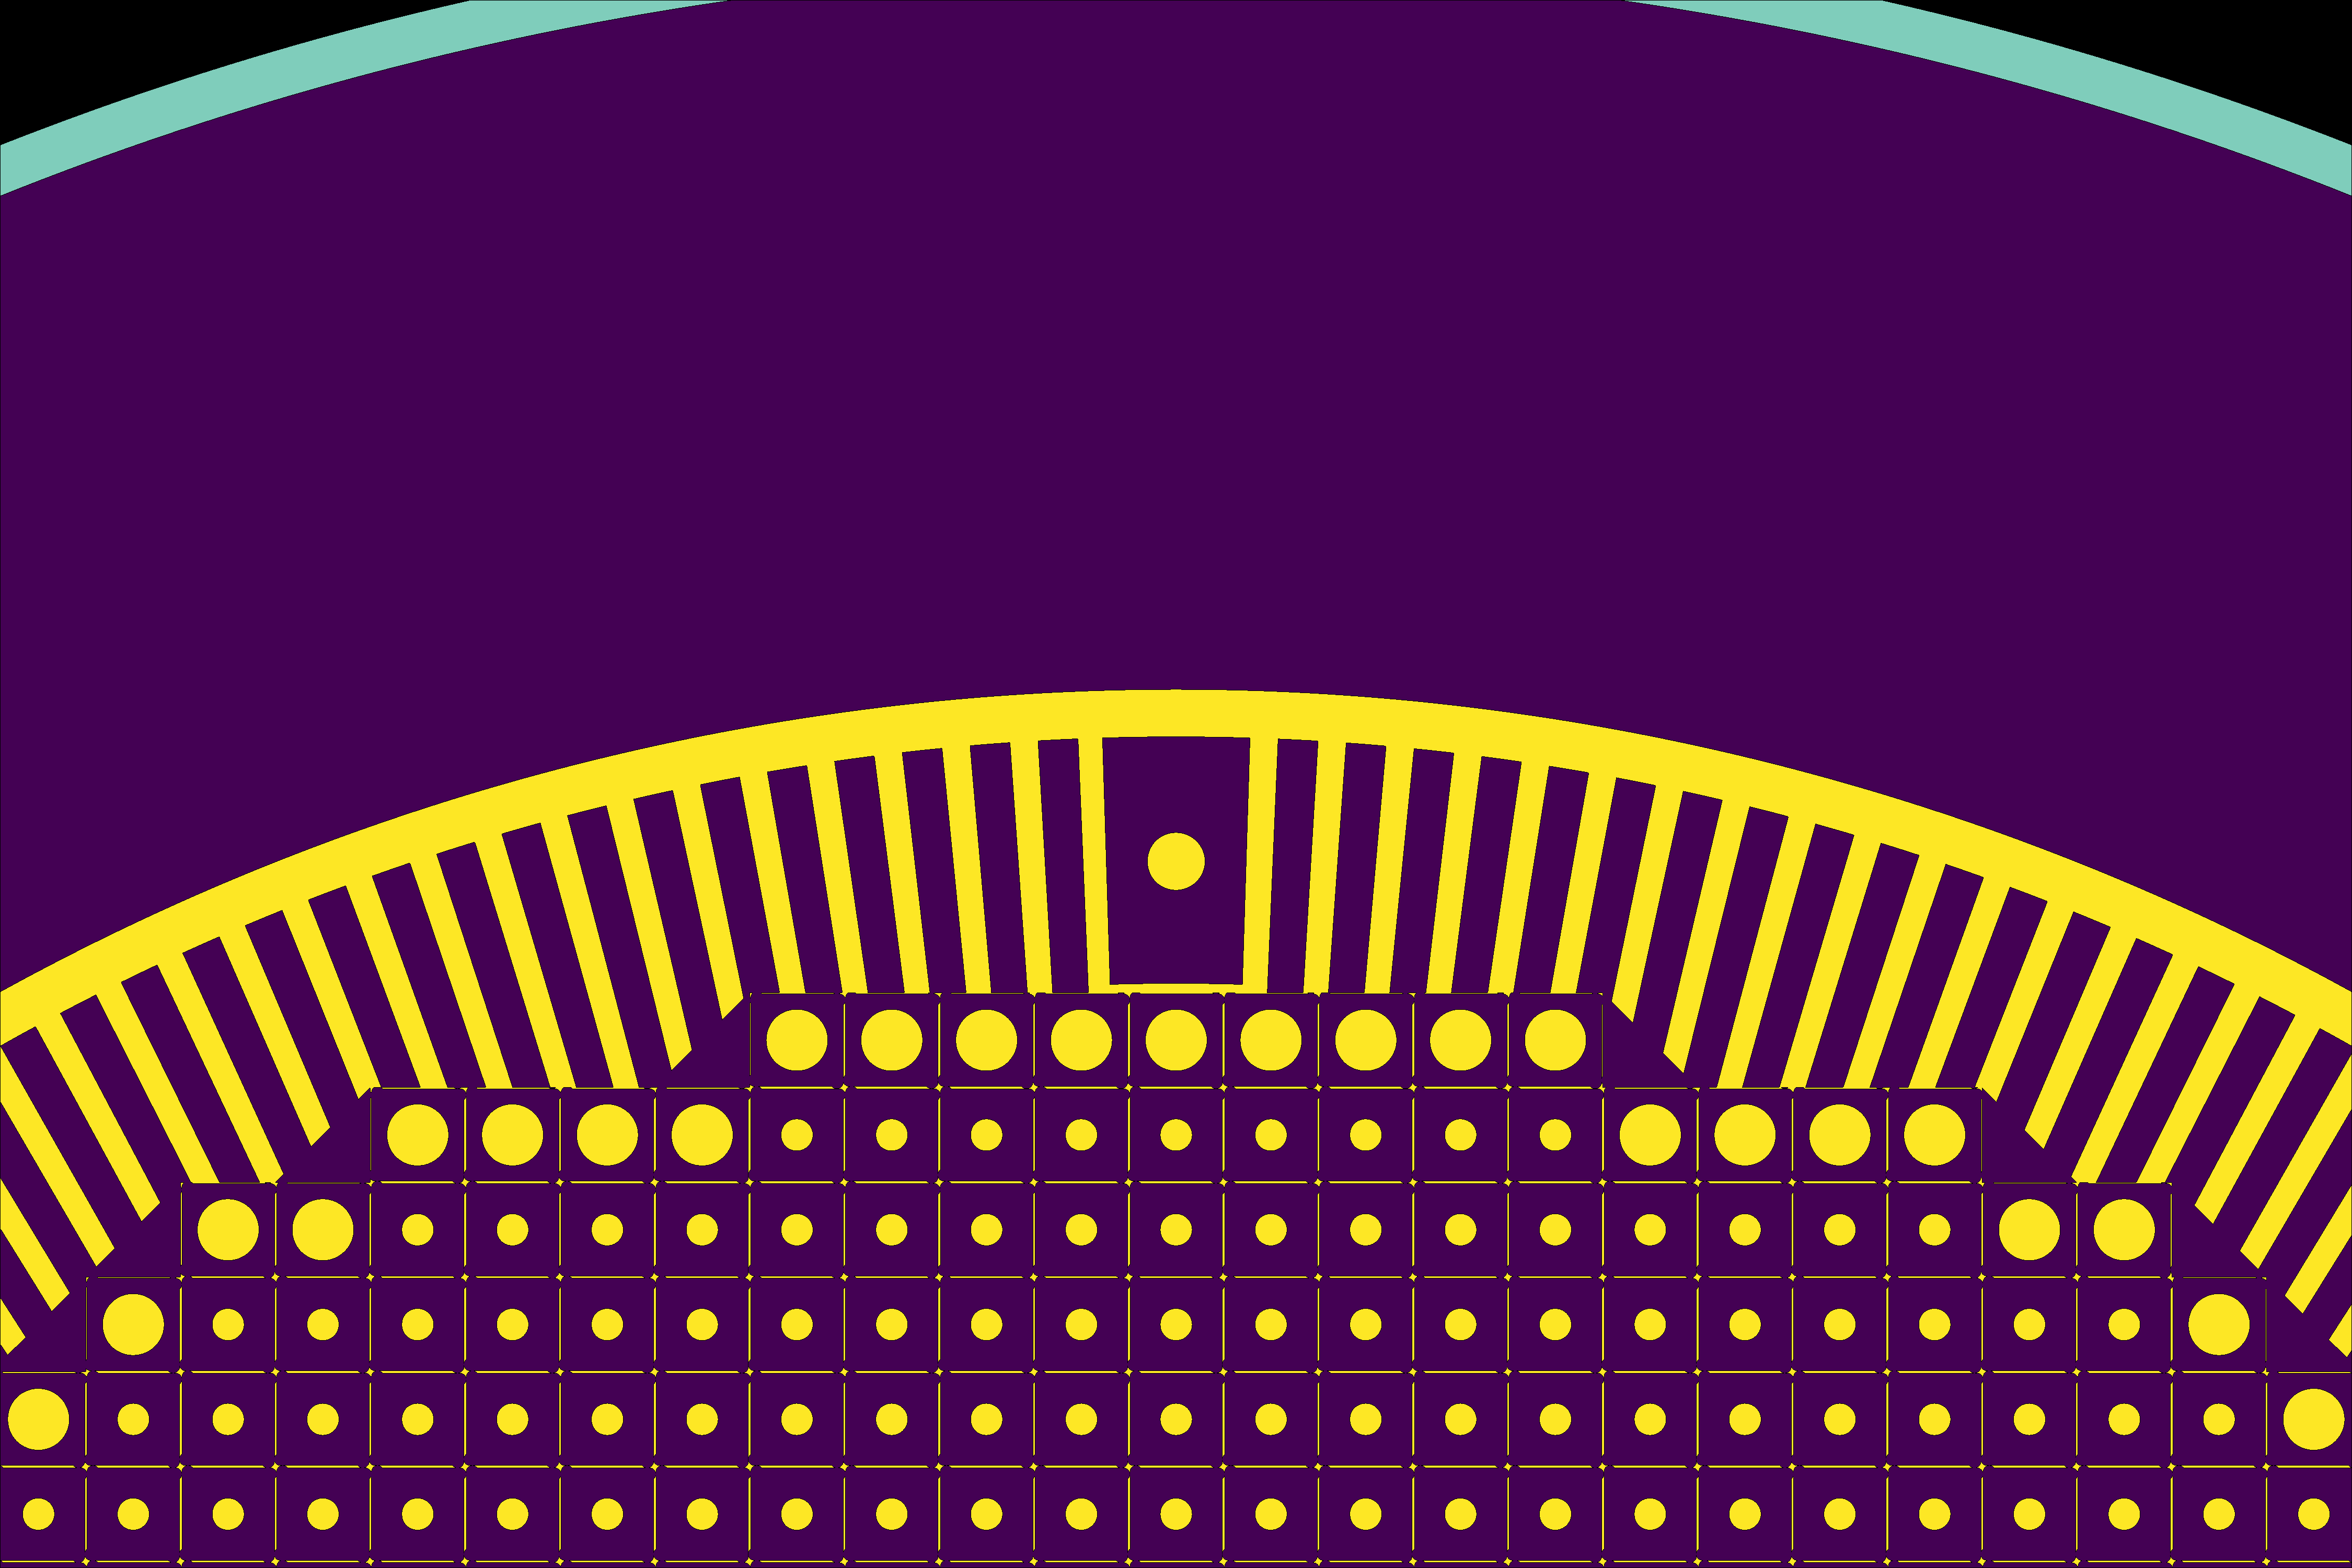
\includegraphics[width=\linewidth]{figure_2_5.png}
  \caption{Plan view of Zone II-B.}
  \label{fig:zone2B}
\end{figure}

%%%%%%%%%%%%%%%%%%%%%%%%%%%%%%%%%%%%%%%%%%%%%%%%%%%%%%%%%%%%%%%%%%%%%%%%%%%%%%%%
\subsection{Subsection Goes Here}
The user must manually capitalize initial letters of a subsection heading.

For those who like equations in their papers, \LaTeX\ is a good choice. Here is
an equation for the Marshak diffusion boundary condition:

shows how a plot might conceivably look in your
document. Always place figures after they are referenced so as not to throw
off the reader. You can use symbols and different line styles to help
differentiate your results, especially if they are printed in black and white.
Note how Fig.~\ref{fig:voltage} uses dashed lines \verb|--| for the exact
solution, solid lines \verb|-| for the new method's solutions, and dotted lines
\verb|:| for existing inaccurate methods.
\begin{figure}[ht] % replace 't' with 'b' to force it to be on the bottom
  \centering
  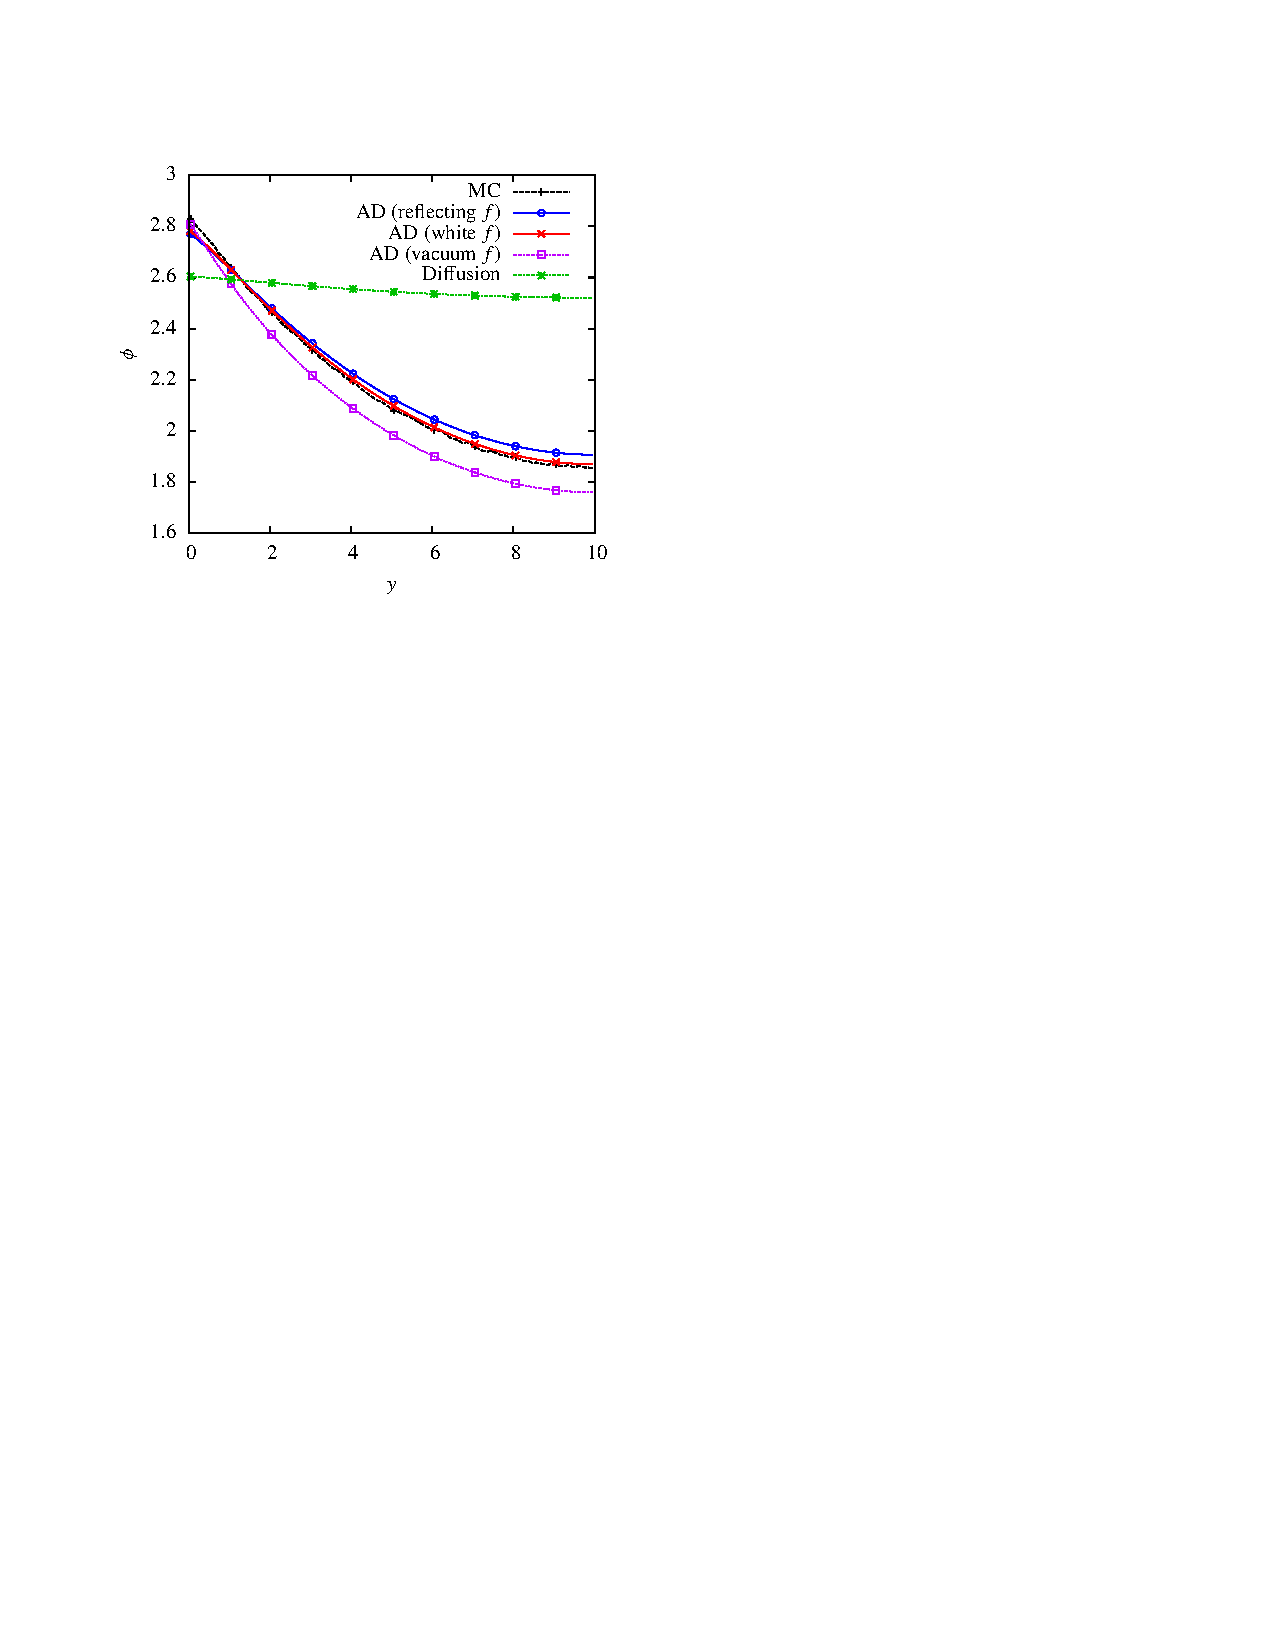
\includegraphics{example_figure}
  \caption{Captions are flush with the left.}
  \label{fig:voltage}
\end{figure}

Later on, we can include a table, even one that spans two columns such as
Table~\ref{tab:widetable}.
%%%%%%%%%%%%%%%%%%%%%%%%%%%%%%%%%%%%%%%%
\begin{table*}[htb]
  \centering
\begin{tabular}{llllllllll}\toprule
      & $\phi_T(0)$      & $\phi_T(10)$      & $\phi_T(20)$      &
      $\phi_D(0)$      & $\phi_D(10)$      & $\phi_D(20)$      & $\rho$      &
      $\varepsilon$      & $N_\text{it}$
\\ \midrule
$c=0.999$  & 0.9038 & 20.63 & 31.24 & 0.9087 & 20.63 & 31.23 & 0.2192 & $10^{-7}$ & 15
\\
$c=0.990$  & 0.3675 & 13.04 & 24.7 & 0.3696 & 13.04 & 24.69 & 0.2184 & $10^{-7}$ & 15
\\
$c=0.900$  & 0.009909 & 4.776 & 17.64 & 0.009984 & 4.786 & 17.63 & 0.2118 & $10^{-7}$ & 14
\\
$c=0.500$  & $6.069\times 10^{-5}$ & 2.212 & 15.53 & 6.213$\times 10^{-5}$ & 2.239 & 15.53 & 0.2068 & $10^{-7}$ & 13
\\
\bottomrule
\end{tabular}
  \caption{This is an example of a really wide table which might not normally
  fit in the document.}
  \label{tab:widetable}
\end{table*}
%%%%%%%%%%%%%%%%%%%%%%%%%%%%%%%%%%%%%%%%
Notice how the table reference uses a Roman numeral
for its numbering scheme, whereas the figure reference uses an Arabic numeral.
For one-column tables, use the \verb|table| environment; two-column tables use
\verb|table*|. The same applies to figures.

%%%%%%%%%%%%%%%%%%%%%%%%%%%%%%%%%%%%%%%%%%%%%%%%%%%%%%%%%%%%%%%%%%%%%%%%%%%%%%%%
\subsection{Another Subsection}
Excessive sectioning in a three-page document is discouraged, but here are more
subsections to demonstrate compliance with the ANS formatting guidelines.

\subsubsection{Third-level Heading}
This subsubsection shows compliance with the ANS-specified standard. This level
of heading should be used rarely.

\subsubsection{Another Such Heading}
And, if you really think you need a third-level heading, you should make sure
that your subsection needs at least two of them.

%%%%%%%%%%%%%%%%%%%%%%%%%%%%%%%%%%%%%%%%%%%%%%%%%%%%%%%%%%%%%%%%%%%%%%%%%%%%%%%%
\section{Conclusions}

The included ANS style file and this clear example file are a panacea for
the hours of headache that invariably results from formatting a document in
Microsoft Word.

%%%%%%%%%%%%%%%%%%%%%%%%%%%%%%%%%%%%%%%%%%%%%%%%%%%%%%%%%%%%%%%%%%%%%%%%%%%%%%%%
\appendix
\section{Appendix}

Numbering in the appendix is different:
\begin{equation} \label{eq:appendix}
  2 + 2 = 5\,.
\end{equation}
and another equation:
\begin{equation} \label{eq:appendix2}
  a + b = c\,.
\end{equation}

%%%%%%%%%%%%%%%%%%%%%%%%%%%%%%%%%%%%%%%%%%%%%%%%%%%%%%%%%%%%%%%%%%%%%%%%%%%%%%%%
\section{Acknowledgments}
This material is based upon work supported a Department of Energy Nuclear
Energy University Programs Graduate Fellowship.

%%%%%%%%%%%%%%%%%%%%%%%%%%%%%%%%%%%%%%%%%%%%%%%%%%%%%%%%%%%%%%%%%%%%%%%%%%%%%%%%
\bibliographystyle{ans}
\bibliography{bibliography}
\end{document}

